\documentclass[10pt,a4paper]{article}
\usepackage[utf8]{inputenc}
\usepackage[spanish]{babel}
\usepackage{amsmath}
\usepackage{amsfonts}
\usepackage{amssymb}
\usepackage{enumitem}
\usepackage{hyperref} 
\usepackage{listings}
\usepackage{graphicx}
\usepackage{amsmath}
\usepackage{listings}
\usepackage{xcolor}
\usepackage{hypcap}
\definecolor{codegreen}{rgb}{0,0.6,0}
\definecolor{codegray}{rgb}{0.5,0.5,0.5}
\definecolor{codepurple}{rgb}{0.58,0,0.82}
\definecolor{backcolour}{rgb}{0.95,0.95,0.92}
\lstdefinestyle{mystyle}{
    backgroundcolor=\color{backcolour},   
    commentstyle=\color{codegreen},
    keywordstyle=\color{magenta},
    numberstyle=\tiny\color{codegray},
    stringstyle=\color{codepurple},
    basicstyle=\ttfamily\footnotesize,
    breakatwhitespace=false,         
    breaklines=true,                 
    captionpos=b,                    
    keepspaces=true,                 
    numbers=left,                    
    numbersep=5pt,                  
    showspaces=false,                
    showstringspaces=false,
    showtabs=false,                  
    tabsize=2
}
\lstset{style=mystyle}
\author{Pablo Riutort Grande}
\title{Seguridad en redes\\ \vspace{1cm}\textbf{Práctica 1}}
\begin{document}
\maketitle
\pagebreak
\section{}
\subsection{}
Los \textit{downloaders} son un tipo de malware especializado cuya funcionalidad es la de descargarse contenido. Se trata de un malware de bajo coste, poco riesgo, reusable y bastante común.\\
El contenido de la descarga suele ser variable: comandos, archivos de configuración, aplicaciones, upgrades, etc. \\
Las pequeñas descargas son más difíciles de detectar que si se tratase de una descarga más grande y, además, reduce el riesgo de fallo. Si fuese detectado por un antivirus, el atacante puede crear otros componentes del \textit{downloader} y reutilizar gran parte de los recursos. \\
El alcance del daño está solo limitado a lo que el malware se pueda descargar.\\

En las capturas de Wireshark podemos observar que siempre se hace una petición a un archivo ``update.zip''.

\begin{figure}[h!]
  \centering
  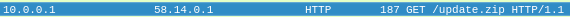
\includegraphics[scale=0.6]{1_1.png}\\
  \caption{Petición de tipo GET del protocolo HTTP a un archivo update.zip}
  \label{fig:get}
\end{figure}

\begin{figure}[h!]
  \centering
  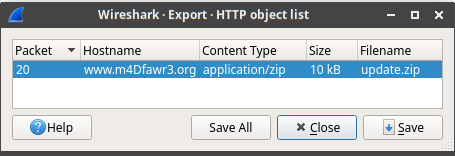
\includegraphics[scale=0.6]{1_1_2.png}\\
  \caption{Exportación de objeto HTTP}
  \label{fig:object}
\end{figure}

Si descargamos este archivo veremos que se trata de un pequeño archivo de 10kB protegido con contraseña.

\begin{figure}[h!]
  \centering
  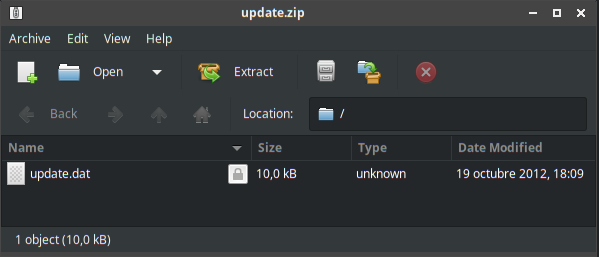
\includegraphics[scale=0.6]{1_1_3.png}\\
  \label{fig:update}
\end{figure}

\begin{figure}[h!]
  \centering
  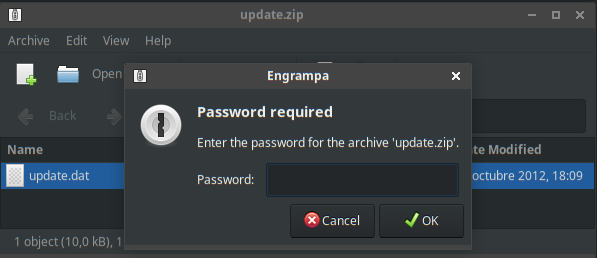
\includegraphics[scale=0.6]{1_1_4.png}\\
    \caption{Contenido del archivo update.zip}
  \label{fig:update2}
\end{figure}

Aparentemente, la descripción del dowloader concuerda con la secuencia y contenido de los paquetes, puesto que se ha descargado un archivo de unos pocos kilobytes de naturaleza sospechosa: llamado ``update'' y protegido por contraseña.

\subsection{}
Los protocolos correspondientes a la capa de aplicación utilizados por el \textit{downloader} son DNS y HTTP.

\begin{figure}[h!]
  \centering
  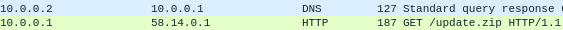
\includegraphics[scale=0.6]{1_2.png}\\
      \caption{Captura de Wireshark mostrando IPs y protocolos implicados}
  \label{fig:http_dns}
\end{figure}

\subsection{}
Para este apartado se ha ejecutado el comando \textit{whois} sobre las direcciones IP referenciadas por el \textit{downloader}:
\begin{itemize}
\item 58.14.0.1
\begin{lstlisting}
inetnum:        58.14.0.0 - 58.15.255.255
netname:        JNGDNET
country:        CN
descr:          Jinan Radio \&TV Wellunited
descr:          Digital Cable TV Co., Ltd
descr:          3F Sanjianyinyuan Building,No.22 minsheng Road
descr:          Jinan, Shandong, P.R.China
...
address:        Beijing, China
\end{lstlisting}
\item 61.29.128.91
\begin{lstlisting}
inetnum:        61.29.128.0 - 61.29.159.255
netname:        CHINANETCENTER
descr:          ChinaNetCenter Ltd.
country:        CN
...
address:        Beijing, China
\end{lstlisting}

\item 123.64.99.200
\begin{lstlisting}
inetnum:        123.64.0.0 - 123.95.255.255
netname:        CTTNET
descr:          China TieTong Telecommunications Corporation
descr:          Jinze Mansion, 2 Guangningbo Street,
descr:          Xicheng District, Beijing, China, 100032
country:        CN
...
address:        Beijing, China
\end{lstlisting}
\item 166.111.111.166
\begin{lstlisting}
inetnum:        166.111.0.0 - 166.111.255.255
netname:        TUNET
descr:          imported inetnum object for IIINT
country:        CN
...
address:        Room 224, Main Building
                Tsinghua University
                Beijing, 100084
\end{lstlisting}
\item 203.100.192.58
\begin{lstlisting}
inetnum:        203.100.192.0 - 203.100.207.255
netname:        ZLLX
descr:          Beijing Zhonglianlixin Technology Co., Ltd.
admin-c:        LH2804-AP
tech-c:         LH2804-AP
country:        CN
...
address:        3F,Building39,Shaoyaoju,Chaoyang District,Beijing, China
\end{lstlisting}

\item 210.14.128.7
\begin{lstlisting}
inetnum:        210.14.128.0 - 210.14.143.255
netname:        SHUJUJIA
descr:          Beijing ShuJuJia Technology Co., Ltd.
descr:          Triumph 170 Kai Xuan Cheng, 26th Floor, Block C
descr:          Bei Yuan Road, Chaoyang District, Beijing City
country:        CN
...
address:        Beijing CNISP Technology Co., Ltd
\end{lstlisting}

\end{itemize}

La procedencia geográfica del malware es de \textbf{Beijing, China}.

\pagebreak

\section{}

\subsection{}
La regla definida para Snort es la siguiente:

\begin{figure}[htpb]
	\lstinputlisting[language=bash]{RiutortSeguridad_redes_LAB1_rule.snort}
    \caption{Regla definida para detectar \textit{downloader} con Snort}
    \label{fig:rule}
\end{figure}

\begin{itemize}
\item \textbf{alert}. Snort puede efectuar varias acciones si se cumple la regla definida: En este caso, generará una acción de tipo ``alert''.
\item \textbf{tcp}. Tipo de paquete sobre el que debe actuar esta regla. En este caso, sobre TCP.
\item \textbf{10.0.0.1 any $\rightarrow$ any any}. Aquí se define el origen, destino y dirección del paquete. En este caso tenemos como IP de origen el de las pcaps: 10.0.0.1. Como IP de destino, puertos de origen y destino pueden ser cualquiera.
\item \textbf{msg:``MISTIC malware trojan detected''}. El ``msg'' configura el engine de logs y de alertas para escribir el mensaje indicado junto al paquete que cumple la regla especificada. En este campo podemos definir concretamente qué mensaje.
\item \textbf{sid:124444}. El ID de la regla.
\item \textbf{rev:1}. El número de revisión de la regla: un control de versión para su correcto mantenimiento.
\item \textbf{priority:4}. El ``priority'' indica mediante un número entero la prioridad de la regla. El rango de prioridades va desde 1 (alto) hasta 4 (muy bajo).
\item \textbf{classtype:trojan-activity}. El ``classtype'' se utiliza para categorizar una regla al detectar un ataque. De esta forma, se puede determinar que el ataque es parte de una clase de ataques. En este caso, la regla lo cataloga como un ataque relacionado con la actividad de un troyano.
\item \textbf{flow:to\_server,established}. El campo ``flow'' permite a la regla aplicarse solo en ciertas direcciones del flujo de tráfico. En este caso, tenemos que la regla se aplica cuando haya peiticiones como cliente en conexiones TCP establecidas.
\item \textbf{content:``User-Agent'';http\_header}. El campo ``content'' permite al usuario configurar las reglas para buscar un contenido especifico en el \textit{payload} del paquete. De esta forma podemos buscar contenido específico en las tramas a analizar. ``content'' permite una serie de palabras clave que matizan la naturaleza del contenido, en este caso, se restringe la búsqueda de la búsqueda a las cabeceras HTTP.
\item \textbf{pcre}. El campo ``pcre'' permite usar expresiones regulares.
\begin{lstlisting}
"/^User-Agent\s*:[^\n]*malw4r3/"
\end{lstlisting}
Esta expresión regular permite buscar en la cabecera ``User-Agent'' del protocolo HTTP el valor que contenga la palabra ``malw4r3'', puesto que es una característica común de todas las pcaps del \textit{downloader} en la petición de descarga del archivo ``update.zip''.

\begin{figure}[h!]
  \centering
  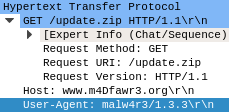
\includegraphics[scale=0.8]{2_1_2.png}
  \caption{Cabecera ``User-Agent'' de la trama GET}
  \label{fig:pcre}
\end{figure}

\end{itemize}

\begin{figure}[h!]
  \centering
  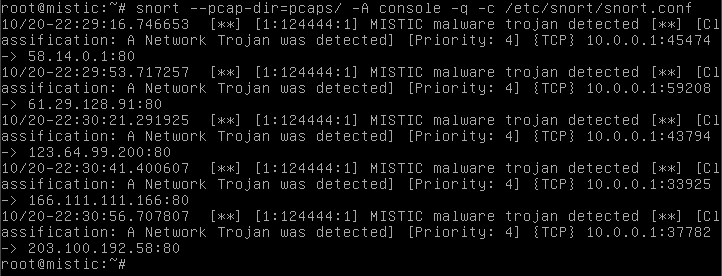
\includegraphics[width=1\textwidth]{2_1.png}
  \caption{Ejecución de Snort con la nueva regla añadida sobre el directorio pcap/}
  \label{fig:snort}
\end{figure}

\pagebreak
\section{}
\subsection{}
Tal como se puede apreciar en la figura \ref{fig:snort} no hay ninguna detección relativa a la sexta pcap cuya IP de destino es 210.14.128.7.
\subsection{}
La muestra número 6 ha conseguido evadir la regla de Snort. De alguna forma, ha evitado que la expresión regular fuera evaluada correctamente en el proceso de detección y por eso no ha activado la alarma.
\subsection{}
Snort no parece mostrar ningún tipo de alerta sospechosa.
\subsection{}
La técnica utilizada por el \textit{downloader} se denominda\textit{Fragmentation reassembly timeout attack} que, tal como su nombre indica, consiste en utilizar la fragmentación de paquetes en el protocolo IP.\\
Dentro del protocolo IP existe la posibilidad de fragmentar el paquete y mandarlo en trozos más pequeños que son reordenados y reconstruidos en el destinatario. Este ataque se puede utilizar de tal forma que se puede eludir las reglas de Snort y el destinatario reordena la trama final ejecutando el ataque.
\begin{figure}[htpb]
  \centering
  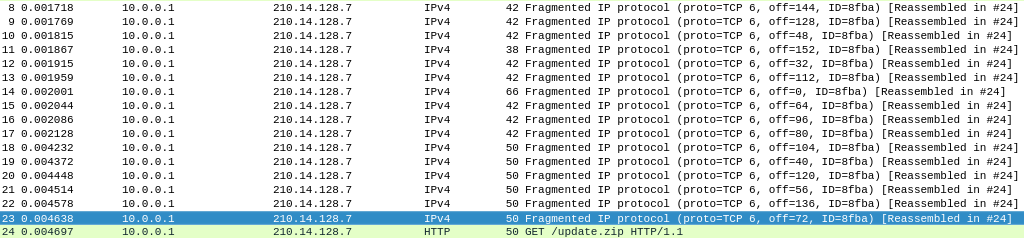
\includegraphics[width=1\textwidth]{3_1.png}
  \caption{Fragmentación de paquetes IP reordenados en la trama 24}
  \label{fig:pcap6}
\end{figure}
Como se puede apreciar, el ataque se divide en distintos fragmentos que son reconstruidos al final. Esta reconstrucción pasa desapercibida para el NIDS y se puede efectuar la descarga del archivo malicioso.
\begin{figure}[htpb]
  \centering
  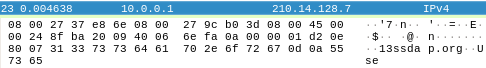
\includegraphics[width=1\textwidth]{3_2_2.png}
  \caption{Contenido de la trama 23}
  \label{fig:pcap6_2}
\end{figure}

\begin{figure}[htpb]
  \centering
  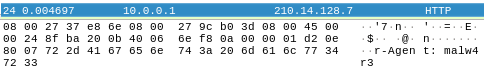
\includegraphics[width=1\textwidth]{3_2_3.png}
  \caption{Contenido de la trama 24}
  \label{fig:pcap6_3}
\end{figure}

Se puede observar que los datos que utilizamos para determinar el contenido malicioso (User-Agent: malw4r3) queda dividido en 2 tramas diferentes (fig. \ref{fig:pcap6_2},  fig. \ref{fig:pcap6_3}) y la expresión regular para detectarlo no tiene efecto.

\subsection{}
\begin{figure}[htpb]
  \centering
  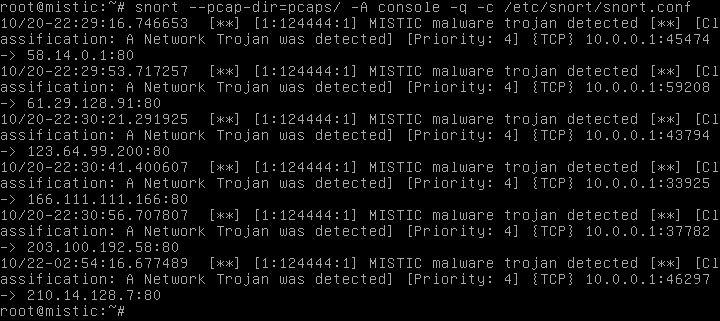
\includegraphics[width=1\textwidth]{3_2.png}
  \caption{Ejecución de Snort con la modificación del preprocesador}
  \label{fig:snort2}
\end{figure}
Al cambiar la política del preprocesador, se cambia la manera en la que se reordenan los fragmentos IP en el NIDS. La política actual reordena las tramas de manera que la expresión regular surge efecto y podemos detecta el texto que nos indica que el paquete es, efectivamente, un malware \textit{downloader}.
\subsection{}
Los preprocesadores permiten ampliar la funcionalidad de Snort de manera modular. Concretamente, los preprocesadores son programas que actúan antes que el motor de detección y después de que el paquete se haya decodificado. De esta forma, el paquete puede ser analizado de manera independiente. El preprocesador \textit{frag3} es un módulo de desfragmentación de IP basado en objetivos (\textit{target-based}).
 
\subsection{}
Por defecto, Snort tiene la política de fragmentación First, correspondiente a la plataforma Windows. Esta política reordena los paquetes por orden de llegada estricto y esta política no podía detectar el ataque. La política de Linux, en cambio, reordena los paquetes de forma diferente, una que sí permite detectar el malware.
\subsection{}
En Snort hay 2 directivas del preprocesador \textit{frag3}, la global y la configuración del motor. En la última, el usuario puede estipular qué política de desfragmentación se tiene que configurar para una IP de destino. \\
El preporcesador de \textit{frag3} es un módulo de desfragmentación para Snort basado en IP objetivo. En un sistema basado en objetivos se modelan los objetivos reales en la red en vez de modelar los protocolos y buscar ataques en ellos. Los ataques IPs se diseñan para distintos sistemas operativos, de esta forma, se puede modelar el sistema objetivo en una situación más realista.

\pagebreak
\section{}
Esta regla detecta una vulnerabilidad en la función ``use\_syslog()'' en el sistema de impresión LPRng v3.6.24 que permite al atacante ejecutar comandos arbitrarios.
\begin{itemize}
\item \textbf{alert}. Generación de una acción de tipo ``alert''.
\item \textbf{tcp}. Tipo de paquete sobre el que debe actuar.
\item \textbf{\$EXTERNAL\_NET any $\rightarrow$ \$HOME\_NET 515}. Dirección del paquete. En este caso cualquier paquete que venga desde el exterior por cualquier puerto hacia la red interna con el puerto 515 como destino.
\item \textbf{msg:``EXPLOIT Redhat 7.0 lprd overflow''}. Mensaje que generará la alerta en caso de cumplirse la regla.
\item \textbf{flow:to\_server,established}. Aplica la regla en conexiones TCP establecidas como cliente.
\item \textbf{content:``XXX\%.172u\%300$\vert$24$\vert$n''}. Busca en la trama este contenido.
\item \textbf{reference:bugtraq,1712}. El campo ``reference'' permiten a la regla incluir referencias a sistemas de identificación de ataques externos. En este caso tenemos una referencia al sistema \href{https://www.securityfocus.com/bid/}{bugtraq}.
\item \textbf{reference:cve,2000-0917}. Esta es otra referencia, en este caso al \href{http://cve.mitre.org/cgi-bin/cvename.cgi?name=}{Common Vulnerabilities and Exposures}.
\item \textbf{classtype:attempted-admin}. La categoría de este ataque pertenece a la clase de intentar ganar privilegios de administrador.
\item \textbf{sid:302}. ID de la regla.
\item \textbf{rev:9}. Número de revisión.
\end{itemize}
La regla busca cualquier trama que venga desde la red externa al puerto 515 cuyo contenido sea: ``XXX\%.172u\%300$\vert$24$\vert$n''.
De esta forma se protege al sistema de que alguien pueda explotar esta vulnerabilidad.

\section{}
\subsection{}
En términos generales el script inicializa una cadena llamada WHITELIST donde se recogen algunas reglas conrcetas. Se inicializan las cadenas por defecto (INPUT, OUTPUT, FORWARD) para que sigan una política de rechazo por defecto (DROP).\\

A continuación se definen una serie de normas para la cadena INPUT que acepta conexiones SSH y rechaza aquellas conexiones que consistan en más de 6 peticiones en 30 segundos. También añade a la WHITELIST una serie de IPs de origen y rechaza todo lo demás en lo relativo a esta cadena.\\

Finalmente añade a la cadena de OUTPUT los paquetes relativos a conexiones en curso.

\subsection{}

\begin{figure}[htpb]
	\lstinputlisting[language=bash]{iptables}

\end{figure}

\begin{figure}[htpb]
	\lstinputlisting[firstline=2,lastline=3,language=bash]{iptables}
        \caption{Vacía (\textit{flush}) todas las cadenas de la tabla y elimina todas las cadenas que no sean por defecto.}
\end{figure}

\begin{figure}[htpb]
	\lstinputlisting[firstline=5,lastline=7,language=bash]{iptables}
    \caption{Configura la política para las cadenas por defecto. En este caso la política es rechazar todo por defecto.}
\end{figure}

\begin{figure}[htpb]
	\lstinputlisting[firstline=8,lastline=9,language=bash]{iptables}
    \caption{Crea una cadena nueva llamada ``WHITELIST''}
\end{figure}

\pagebreak

A continuación todos los comandos hacen referencia a la acción de añadir reglas a una u otra cadena (-A).\\

En esta sección, concretamente, hablamos siempre de añadir reglas a la cadena por defecto de INPUT. Esta cadena hace referencia a todo el tráfico de entrada.
\begin{figure}[htpb]
	\lstinputlisting[firstline=10,lastline=10,language=bash]{iptables}
    \caption{Se acepta tráfico que provenga de la interface de loopback.}
\end{figure}

\begin{figure}[htpb]
	\lstinputlisting[firstline=12,lastline=12,language=bash]{iptables}
    \caption{Se aceptan paquetes que pertenezcan a conexiones ya existentes y a paquetes que estén relacionados a las mismas como los errores ICMP. El flag \textbf{-m} en iptables sirve para cargar extensiones que ayudan a determinar la naturaleza del paquete. El flag junto con la extensión hacen una comparación con el paquete. Por ejemplo, en la siguiente regla tenemos el state \textbf{NEW} que lo que hará será permitir evaluar el paquete con la extensión \textbf{NEW} que nos dice si el paraquete crea una nueva conexión.}
\end{figure}

\begin{figure}[htpb]
	\lstinputlisting[firstline=13,lastline=13,language=bash]{iptables}
    \caption{Todo paquete del protocolo TCP cuyo destino sea el puerto SSH se redirige a la cadena WHITELIST}
\end{figure}

\begin{figure}[htpb]
	\lstinputlisting[firstline=14,lastline=14,language=bash]{iptables}
    \caption{Todo paquete del protocolo TCP cuyo destino sea el puerto SSH y que el paquete cree una nueva conexión. Además, busca en la cadena la IP del paquete y la actualiza o, si no la encuentra, la añade.}
\end{figure}

\begin{figure}[htpb]
	\lstinputlisting[firstline=15,lastline=15,language=bash]{iptables}
    \caption{El estado \textbf{recent} permite crear una lista dinámica de IPs y luego hacer búsquedas en ella de distintas formas. El flag \textbf{update} mira si el paquete se encuentra actualmente en la lista y, si lo está, actualiza su timestamp. El flag \textbf{seconds} delimita la búsqueda a paquetes de la lista que hayan sido actualizados en la franja de segundos indicada. El flag \textbf{hitcount} delimita aún más la búsqueda a paquetes que hayan recibido un valor mayor o igual a este. \textbf{-j LOG} salta a la acción de LOG. Los paquetes que cumplan estas condiciones quedan logueados en el sistema de logs.}
\end{figure}

\begin{figure}[htpb]
	\lstinputlisting[firstline=16,lastline=16,language=bash]{iptables}
    \caption{Es la misma instrucción que antes, sólo que esta vez la acción es de \textbf{DROP}. Es decir, los paquetes quedan primero logueados e inmediatamente después se descartan}
\end{figure}

\begin{figure}[htpb]
	\lstinputlisting[firstline=17,lastline=17,language=bash]{iptables}
    \caption{Paquetes del protocolo TCP cuyo destino sean el puerto SSH y que inicen una nueva conexión serán aceptados.}
\end{figure}

\begin{figure}[htpb]
	\lstinputlisting[firstline=19,lastline=22,language=bash]{iptables}
    \caption{Mete en la WHITELIST la regla que permite que los paquetes cuyo origen sean 10.0.0.0/16, 10.1.0.0/16, 10.2.0.0/16, 10.3.0.0/16 sean redirigidos a la siguiente regla de la cadena que ha sido llamada previamente a esta}
\end{figure}

\begin{figure}[htpb]
	\lstinputlisting[firstline=23,lastline=23,language=bash]{iptables}
    \caption{Si se llega a esta regla en WHITELIST, quiere decir que se rechazan los paquetes.}
\end{figure}

\begin{figure}[htpb]
	\lstinputlisting[firstline=25,lastline=25,language=bash]{iptables}
    \caption{Añade a la cadena de salida la regla que acepta aquellos paquetes que inicien una conexión relacionada con una conexión existente o relacionados con una conexión donde se hayan visto paquetes en ambas direcciones.}
\end{figure}

Recordemos que las reglas se evalúan de arriba abajo. Empezamos con las reglas de creación de WHITELIST y configuración de políticas por defecto. Luego se añaden las reglas que permiten aceptar paquetes de manera siendo cada vez más concretas restrictivas. Primero se especifican las reglas de la cadena INPUT que tienen relación con el protocolo SSH y conexiones previamente establecidas, después se añaden a la lista blanca los paquetes cuyo origen sean unas IPS concretas y se rechazan los demás. Finalmente, a la lista de salidas las conexiones previamente establecidas.

\pagebreak
\subsection{}
El comando que permitiría registrar conexiones SSH que no estén dentro de la lista blanca sería
\begin{lstlisting}
iptables -A WHITELIST -p tcp --dport ssh -j LOG
\end{lstlisting}
y se tendría que situar antes de la regla que rechaza los paquetes que no cumplan algunas de las condiciones anteriores:
\begin{lstlisting}
iptables -A WHITELIST -j DROP
\end{lstlisting}

\end{document}
